\section{下板验证}

\subsection{烧录流程}

下板验证按以下步骤进行：

\begin{enumerate}[leftmargin=2em]
    \item \textbf{烧录OS.bin到SPI Flash}：使用Vivado的Hardware Manager将\texttt{OS.bin}烧录到SPI Flash中。
    \item \textbf{打开串口终端并下载比特流}：在PC端打开SuperCom，配置为COM3、4800波特率、8位数据位、无校验、1位停止位。通过Vivado将生成的比特流文件下载到FPGA开发板。
    \item \textbf{观察输出}：系统上电后，BootLoader从Flash取指执行，将$\mu$C/OS-II搬移到DDR2，然后跳转执行。串口终端应收到系统启动日志。
\end{enumerate}

\subsection{验证结果}

\subsubsection{串口输出}

比特流下载后，SuperCom成功收到$\mu$C/OS-II的完整启动日志：

\begin{figure}[H]
    \centering
    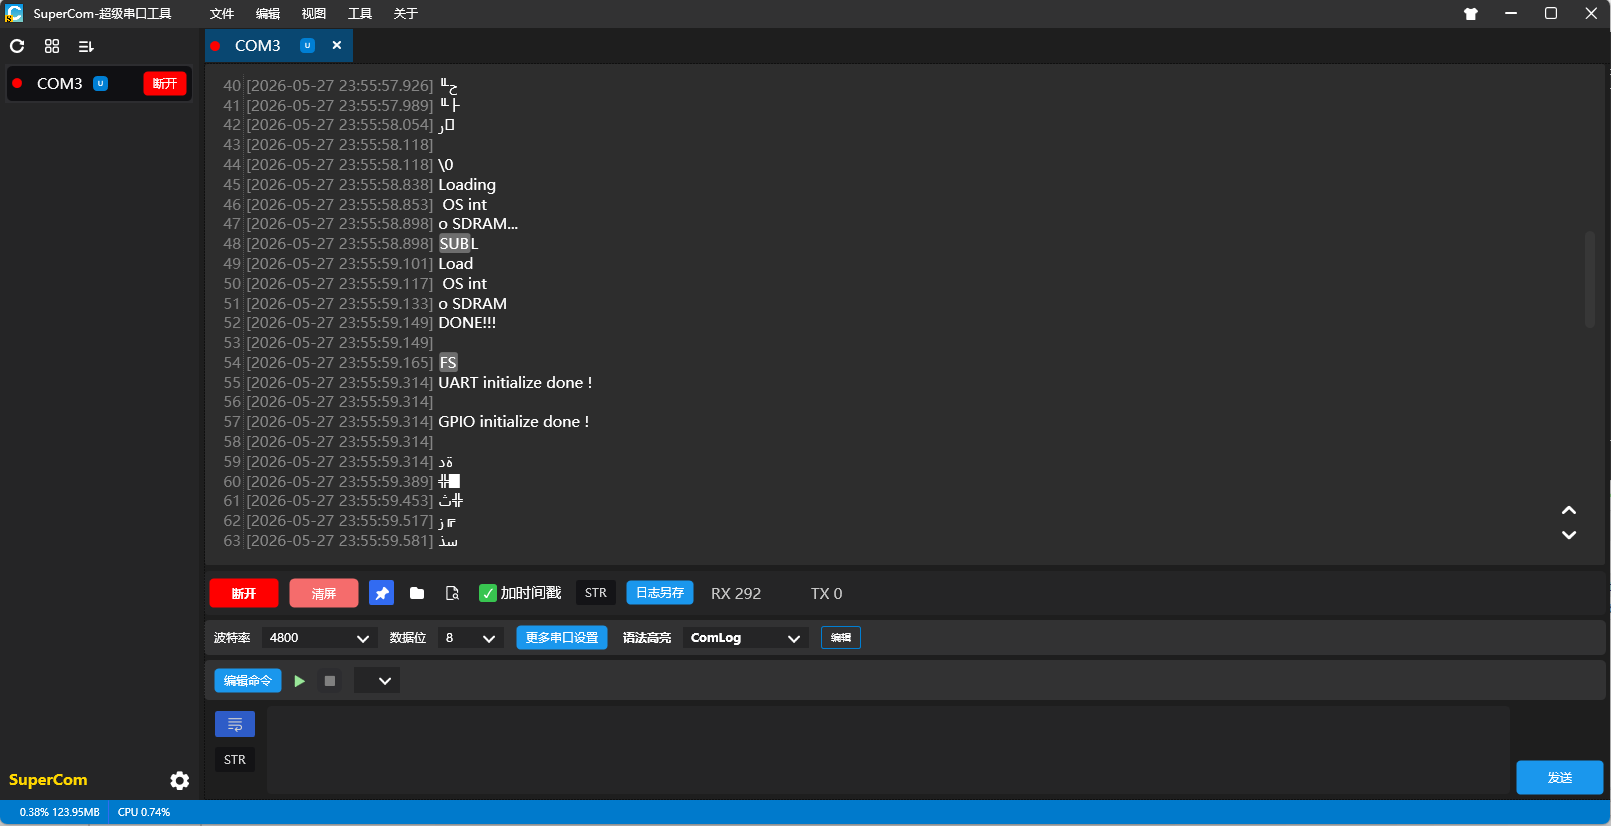
\includegraphics[width=0.85\textwidth]{img/supercom.png}
    \caption{SuperCom串口配置与$\mu$C/OS-II启动输出}
\end{figure}

输出内容清晰可读，说明：
\begin{itemize}[leftmargin=2em]
    \item BootLoader成功从SPI Flash读取并搬移OS映像到DDR2 SDRAM（"Loading OS into SDRAM... DONE!!!"）。
    \item $\mu$C/OS-II成功启动并完成UART初始化（"UART initialize done !"）。
    \item $\mu$C/OS-II成功完成GPIO初始化（"GPIO initialize done !"）。
\end{itemize}

\subsubsection{数码管显示}

$\mu$C/OS-II启动后，数码管以相同频率整齐递增（11111111 $\to$ 22222222 $\to$ ...），说明CPU正在连贯正确地执行用户任务，GPIO模块工作正常。

\begin{figure}[H]
    \centering
    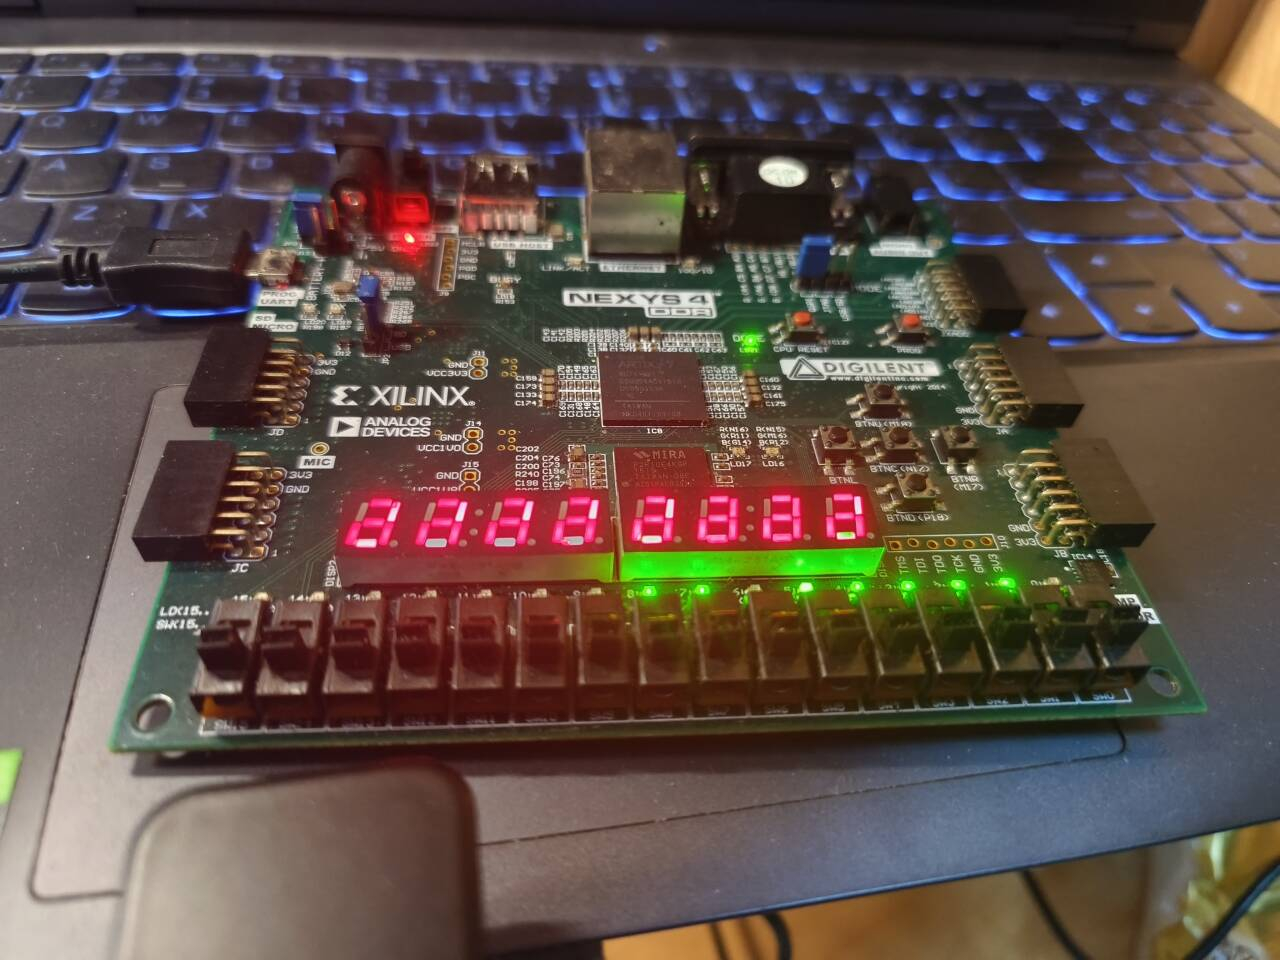
\includegraphics[width=0.45\textwidth]{img/实物1.jpg}
    \caption{数码管递增显示（GPIO正常工作）}
\end{figure}

\begin{figure}[H]
    \centering
    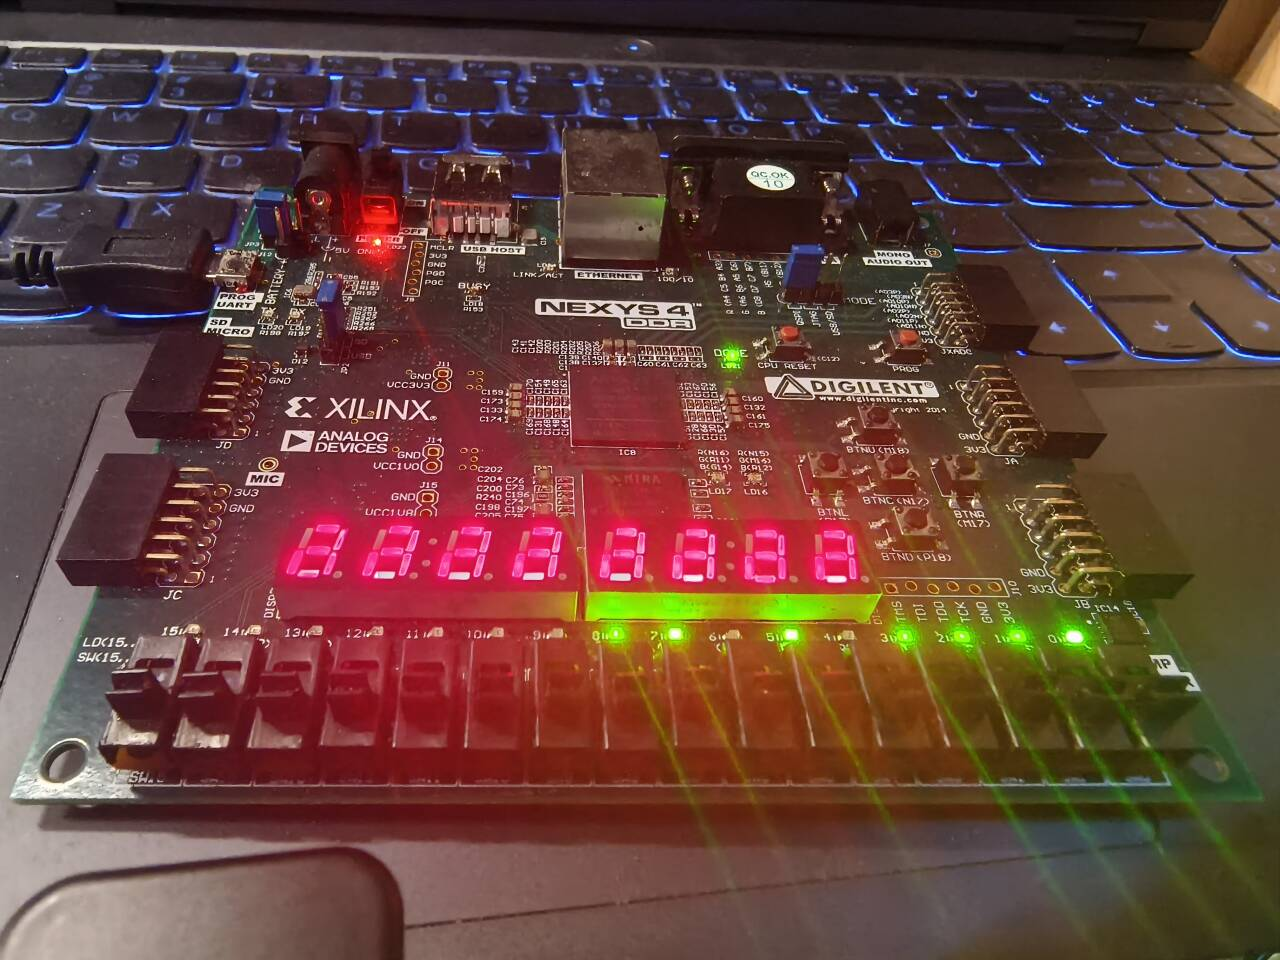
\includegraphics[width=0.45\textwidth]{img/实物3.jpg}
    \caption{数码管显示变化（运行中）}
\end{figure}

\subsubsection{LED状态指示}

开发板上的9个LED用于指示系统运行状态：

\begin{table}[H]
    \centering
    \caption{LED运行状态指示}
    \begin{tabular}{llll}
        \toprule
        \textbf{LED} & \textbf{含义} & \textbf{预期状态} & \textbf{说明} \\
        \midrule
        LD0 & 心跳（$\sim$0.75 Hz） & 慢闪 & 系统时钟正常 \\
        LD1 & CPU取指活动 & 常亮 & CPU从Flash取指正常 \\
        LD2 & UART访问 & 常亮 & CPU已访问UART \\
        LD3 & DDR2初始化完成 & 常亮 & DDR2校准完成 \\
        LD4--LD7 & 跑马灯 & 流水闪烁 & CPU正常运行 \\
        LD8 & UART实时发送 & 随串口闪烁 & 串口数据发送中 \\
        \bottomrule
    \end{tabular}
\end{table}

\begin{figure}[H]
    \centering
    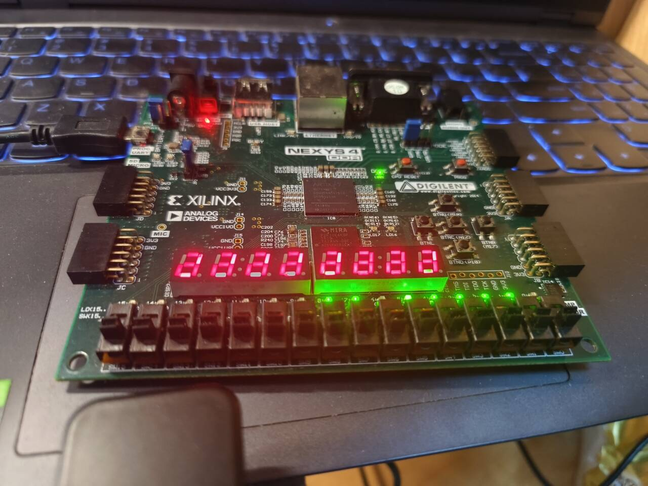
\includegraphics[width=0.45\textwidth]{img/实物2.jpg}
    \caption{LED运行状态指示（LD1/2/3常亮）}
\end{figure}

所有LED状态均符合预期，验证了从Flash取指、DDR2初始化、UART通信和GPIO输出全链路功能正确。
